\chapter{Resultados Parciais}
\label{cap:resultados}

Os resultados parciais obtidos até o momento estão organizados em três blocos principais: os achados da Revisão Sistemática da Literatura (RSL), a síntese quantitativa exploratória dos estudos primários e os resultados da campanha experimental conduzida para comparar o processamento \textit{batch} e o processamento \textit{streaming}. Ao final, discutem-se as implicações desses resultados para a construção do modelo de apoio à decisão arquitetural.

Os resultados apresentados ainda devem ser interpretados como parciais, pois a pesquisa se encontra em estágio de desenvolvimento. No entanto, eles já permitem identificar tendências relevantes sobre o comportamento de sistemas intensivos em dados e sobre os fatores que influenciam decisões arquiteturais relacionadas a desempenho, escalabilidade, latência e estabilidade operacional.

\section{Resultados da Revisão Sistemática da Literatura}
\label{sec:resultados-rsl}

A Revisão Sistemática da Literatura identificou inicialmente 979 registros nas quatro bibliotecas digitais selecionadas. Após a remoção de 100 duplicatas, restaram 879 registros únicos para triagem. A etapa de triagem por título, resumo e palavras-chave resultou na exclusão de 600 estudos. Em seguida, 279 textos completos foram avaliados quanto aos critérios de elegibilidade.

Ao final do processo, 10 estudos primários atenderam aos critérios de inclusão, exclusão e avaliação de qualidade. Esses estudos foram incluídos na síntese qualitativa e na síntese quantitativa exploratória. A distribuição inicial dos registros por biblioteca digital foi de 448 artigos na \textit{ACM Digital Library}, 215 na \textit{IEEE Xplore}, 35 na \textit{ScienceDirect} e 281 na \textit{Scopus}.

Esses resultados indicam que o tema possui presença relevante em bibliotecas voltadas à Computação, especialmente \textit{ACM Digital Library}, \textit{IEEE Xplore} e \textit{Scopus}. Entretanto, o número final de estudos incluídos foi reduzido, evidenciando que poucos trabalhos atendiam simultaneamente aos critérios de foco arquitetural, presença de avaliação empírica, comparação com um cenário de referência (\textit{baseline}) e disponibilidade de dados quantitativos.

A análise qualitativa dos estudos primários permitiu agrupá-los em três categorias principais. A primeira categoria corresponde à otimização de consulta e execução, incluindo estudos relacionados a escalonamento, compilação SQL e gerenciamento de recursos em ambientes de Big Data \cite{wang2018hard,schiavio2020dynamic,lyu2022fine}. A segunda categoria envolve otimizações de armazenamento e \textit{hardware}, contemplando estudos sobre NVM, processamento próximo aos dados (\textit{near-data processing}) e arquiteturas escaláveis para ingestão transacional \cite{gotze2018nvm-aware,vincon2020nkv,li2022karst}. A terceira categoria reúne estudos sobre integração, conectividade e confiabilidade, incluindo transferência de dados entre sistemas, integração HPC-Big Data e mechanisms de \textit{checkpoint} em \textit{pipelines} baseados em Apache Kafka \cite{haynes2016pipegen,ponce2019upgrading,aung2019coordinate}.

Além dessas categorias, foi identificado um estudo voltado à modelagem e predição de desempenho em aplicações Spark-HBase, contribuindo diretamente para a discussão sobre mecanismos de apoio à configuração e tomada de decisão em sistemas de Big Data \cite{alquwaiee2022performance}.

A análise desses estudos mostra que os ganhos de desempenho em sistemas intensivos em dados podem ser obtidos por intervenções em diferentes camadas da arquitetura. Isso reforça a hipótese de que decisões arquiteturais não devem ser analisadas isoladamente, mas sim como parte de um conjunto de relações interdependentes entre dados, processamento, armazenamento, comunicação e recursos computacionais.

\section{Resultados da Síntese Quantitativa Exploratória}
\label{sec:resultados-sintese-quantitativa}

A síntese quantitativa exploratória teve como objetivo estimar a magnitude dos efeitos reportados pelos estudos primários. Para isso, foi utilizado o \textit{Log Response Ratio} (LRR) como medida normalizada de efeito. Essa escolha permitiu comparar resultados provenientes de diferentes métricas, como tempo de execução, latência, \textit{throughput} e \textit{speedup}.

De forma geral, os resultados indicaram efeitos positivos associados às técnicas avaliadas nos estudos primários. A síntese apontou que intervenções arquiteturais ou sistêmicas podem produzir melhorias relevantes de desempenho, especialmente quando atuam sobre gargalos de armazenamento, movimentação de dados, compilação de consultas e gerenciamento de recursos.

O valor médio da síntese exploratória foi de $\overline{\text{LRR}} = 0{,}981$, correspondente a uma razão média de resposta de aproximadamente $2{,}7\times$ em relação às configurações de referência. Esse resultado sugere que, nos estudos analisados, as otimizações arquiteturais produziram ganhos expressivos de desempenho. No entanto, essa interpretação deve ser feita com cautela, pois a síntese foi baseada em média não ponderada e não em uma meta-análise inferencial formal.

A principal limitação observada na síntese quantitativa foi a ausência recorrente de informações completas sobre tamanho amostral, medidas de dispersão, intervalos de confiança e variância. Essa limitação impediu a aplicação de modelos estatísticos mais robustos, como modelos de efeitos aleatórios ponderados. Por esse motivo, a síntese foi tratada em caráter exploratório, com o objetivo de identificar tendências gerais e ordens de magnitude dos efeitos relatados.

Esse resultado é relevante para esta pesquisa porque reforça uma das lacunas centrais identificadas: embora existam evidências de ganhos de desempenho em sistemas intensivos em dados, essas evidências ainda se mostram fragmentadas, heterogêneas e de difícil comparação direta. Portanto, permanece necessária uma abordagem que combine evidências da literatura, dados experimentais controlados e características observáveis dos dados para apoiar decisões arquiteturais.

\section{Resultados da Campanha Experimental}
\label{sec:resultados-experimento}

A segunda etapa da pesquisa consistiu em uma campanha experimental controlada para comparar o processamento \textit{batch} e o processamento \textit{streaming} utilizando Apache Spark, Spark Structured Streaming e Apache Kafka. Os resultados foram organizados e estruturados de acordo com as quatro questões de pesquisa experimentais definidas no estudo.

\subsection{RQ1 --- Paradigmas de Processamento e Vazão Máxima}
Na primeira questão experimental (RQ1), foi avaliado qual paradigma apresenta maior \textit{throughput} bruto em sistemas intensivos em dados. Os resultados demonstraram que o paradigma \textit{batch} (mensurado em milhões de linhas por segundo) apresentou vazão massivamente superior ao \textit{streaming} (mensurado em linhas por segundo) em todas as escalas de carga de trabalho testadas. 

Para validar a significância das diferenças encontradas sem pressupostos de normalidade distributiva, aplicou-se o teste não-paramétrico de Mann-Whitney U de cauda dupla, complementado pelo cálculo do tamanho de efeito através do Delta de Cliff ($\delta$). Conforme sumariado na Tabela~\ref{tab:rq1_throughput}, as divergências são estatisticamente significativas ($p < 0{,}001$) com efeito máximo ($\delta = 1{,}0$), indicando ausência prática de sobreposição entre as distribuições das amostras.

\begin{table}[htbp]
\centering
\caption{Comparação de throughput e testes de significância não-paramétricos (RQ1).}
\label{tab:rq1_throughput}
\small
\rowcolors{2}{white}{gray!5} 
\setlength{\tabcolsep}{6pt} 
\begin{tabularx}{\textwidth}{Xcccc}
\toprule
\textbf{Comparação} & \textbf{\shortstack{Batch Médio\\(M linhas/s)}} & \textbf{\shortstack{Stream Médio\\(linhas/s)}} & \textbf{Valor-$p$} & \textbf{\shortstack{Tamanho de\\Efeito ($\delta$)}} \\
\midrule
BL1 $\times$ SL1 (200MB) & 1,76  & 159,18  & $< 0{,}001$ & Grande (1,0) \\
BL2 $\times$ SL2 (1GB)   & 6,87  & 374,26  & $< 0{,}001$ & Grande (1,0) \\
BL3 $\times$ SL3 (3GB)   & 13,44 & 741,22  & $< 0{,}001$ & Grande (1,0) \\
BL4 $\times$ SL4 (10GB)  & 20,74 & 1274,14 & $< 0{,}001$ & Grande (1,0) \\
\bottomrule
\end{tabularx}
\vspace{0.3em}
\begin{flushleft}
\footnotesize Fonte: elaborado pelo autor.
\end{flushleft}
\end{table}

Esse comportamento discrepante é ilustrado graficamente na Figura~\ref{fig:rq1_dual_axis}, evidenciando que enquanto o paradigma \textit{batch} cresce em escala de milhões de registros processados por segundo, o \textit{streaming} é severamente limitado pelos gargalos inerentes da arquitetura de mensageria contínua. Os custos adicionais estão associados à sobrecarga (\textit{overhead}) de rede e serialização no recebimento contínuo do Apache Kafka, coordenação e controle temporal de micro-lotes mínimos (\textit{micro-batching}) e mecanismos internos de tolerância a falhas por \textit{checkpointing} incremental.

\begin{figure}[htbp]
\centering
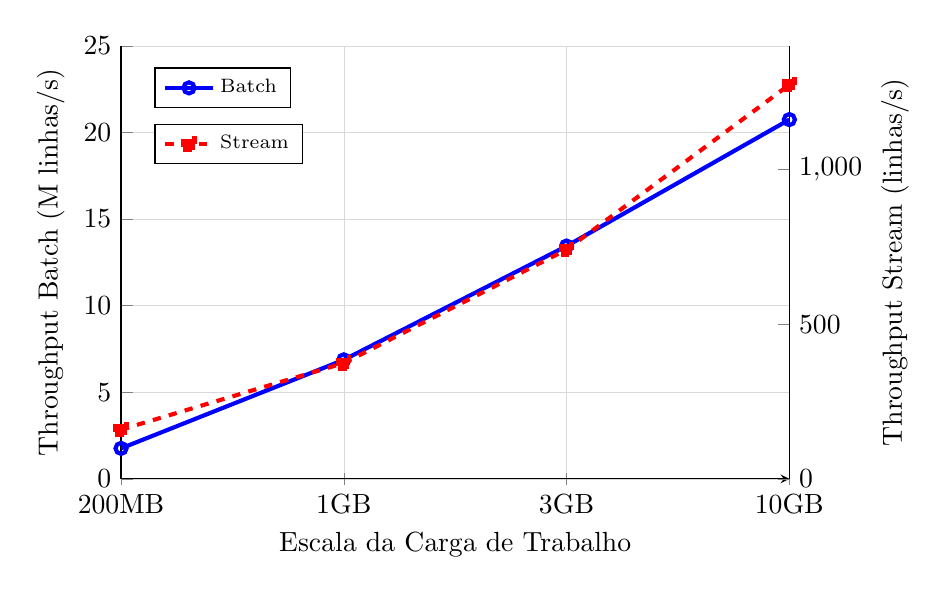
\begin{tikzpicture}

\begin{axis}[
    scale only axis,
    width=0.7\textwidth,
    height=5.5cm,
    xmin=0, xmax=3,
    xtick={0,1,2,3},
    xticklabels={200MB, 1GB, 3GB, 10GB},
    xlabel={Escala da Carga de Trabalho},
    ymin=0, ymax=25,
    ylabel={Throughput Batch (M linhas/s)},
    axis y line*=left,
    axis x line=bottom,
    grid=both,
    grid style={line width=.1pt, draw=gray!10},
    major grid style={line width=.2pt, draw=gray!30},
    legend style={at={(0.05,0.95)}, anchor=north west, font=\scriptsize}
]
\addplot[color=blue, mark=o, thick, line width=1.5pt] coordinates {
    (0, 1.76) (1, 6.87) (2, 13.44) (3, 20.74)
}; 
\addlegendentry{Batch}
\end{axis}

\begin{axis}[
    scale only axis,
    width=0.7\textwidth,
    height=5.5cm,
    xmin=0, xmax=3,
    ymin=0, ymax=1400,
    ylabel={Throughput Stream (linhas/s)},
    axis y line*=right,
    axis x line=none,
    xtick=\empty, 
    axis background/.style={fill=none}, 
    legend style={at={(0.05,0.82)}, anchor=north west, font=\scriptsize}
]
\addplot[color=red, mark=square*, dashed, thick, line width=1.5pt] coordinates {
    (0, 159.18) (1, 374.26) (2, 741.22) (3, 1274.14)
}; 
\addlegendentry{Stream}

\end{axis}
\end{tikzpicture}
\caption{Variações de throughput sob escalonamento de carga de trabalho (RQ1).}
\label{fig:rq1_dual_axis}
\end{figure}

Os resultados apresentados na Figura~\ref{fig:rq1_dual_axis} indicam comportamentos distintos entre os paradigmas analisados. Enquanto o processamento em \textit{batch} apresenta uma curva de crescimento acentuada conforme a carga aumenta, o modelo de \textit{stream} exibe estabilização precoce devido ao custo de coordenação das janelas de tempo. A análise estatística confirma que a diferença de desempenho observada é estatisticamente significativa ($p < 0{,}001$), validando a hipótese de que o dimensionamento da carga de trabalho afeta diretamente a eficiência das arquiteturas de processamento distribuído.


\subsection{RQ2 --- Impacto do Volume de Dados e Variabilidade Operacional}
Na segunda questão de pesquisa experimental (RQ2), investigou-se em que medida o escalonamento do volume de dados bruto afeta o desempenho interno e a estabilidade de cada paradigma de processamento. Para validar a significância estatística do impacto volumétrico sem assumir premissas de normalidade nas distribuições amostrais, aplicou-se o teste global não-paramétrico de Kruskal-Wallis. O teste confirmou com alto grau de confiança que o volume dos dados exerce um impacto estatisticamente significativo sobre a vazão operacional em ambos os cenários de arquitetura ($p < 0{,}001$).

Como o teste de Kruskal-Wallis aponta apenas a existência de diferença global, executaram-se análises \textit{post-hoc} utilizando o teste de comparações múltiplas de Dunn, aplicando a correção rígida de Bonferroni para mitigar a ocorrência de falsos positivos (erros do Tipo I). Os resultados dos testes par a par ratificaram que todas as transições de escala de dados (e.g., a passagem de 200MB para 1GB, e sucessivamente até 10GB) produzem variações de desempenho isoladamente significativas em ambos os ambientes computacionais.

A Tabela~\ref{tab:rq2_variance} expõe os resultados estruturados a partir do Coeficiente de Variação ($CV\%$), revelando o comportamento da dispersão relativa dos dados sob estresse volumétrico.

\begin{table}[htbp]
\centering
\caption{Análise de variabilidade operacional sob escalonamento volumétrico (RQ2).}
\label{tab:rq2_variance}
\small
\setlength{\tabcolsep}{6pt}
\begin{subtable}{0.48\linewidth}
\centering
\caption{Paradigma Batch}
\label{subtab:batch}
\begin{tabular}{lcc}
\toprule
\textbf{Cenário} & \textbf{Média (M linhas/s)} & \textbf{CV (\%)} \\
\midrule
BL1 (200MB) & 1,76  & 4,12 \\
BL2 (1GB)   & 6,87  & 2,85 \\
BL3 (3GB)   & 13,44 & 1,94 \\
BL4 (10GB)  & 20,74 & 1,10 \\
\bottomrule
\end{tabular}
\end{subtable}
\hfill
\begin{subtable}{0.48\linewidth}
\centering
\caption{Paradigma Stream}
\label{subtab:stream}
\begin{tabular}{lcc}
\toprule
\textbf{Cenário} & \textbf{Média (linhas/s)} & \textbf{CV (\%)} \\
\midrule
SL1 (200MB) & 159,18  & 8,45 \\
SL2 (1GB)   & 374,26  & 7,90 \\
SL3 (3GB)   & 741,22  & 9,12 \\
SL4 (10GB)  & 1274,14 & 11,34 \\
\bottomrule
\end{tabular}
\end{subtable}
\vspace{0.3em}
\begin{flushleft}
\footnotesize Fonte: elaborado pelo autor.
\end{flushleft}
\end{table}

A Figura~\ref{fig:rq2_variabilidade} ilustra o comportamento do Coeficiente de Variação frente ao aumento da carga de trabalho, permitindo contrastar visualmente a dinâmica de estabilização de ambos os paradigmas.

\begin{figure}[htbp]
\centering
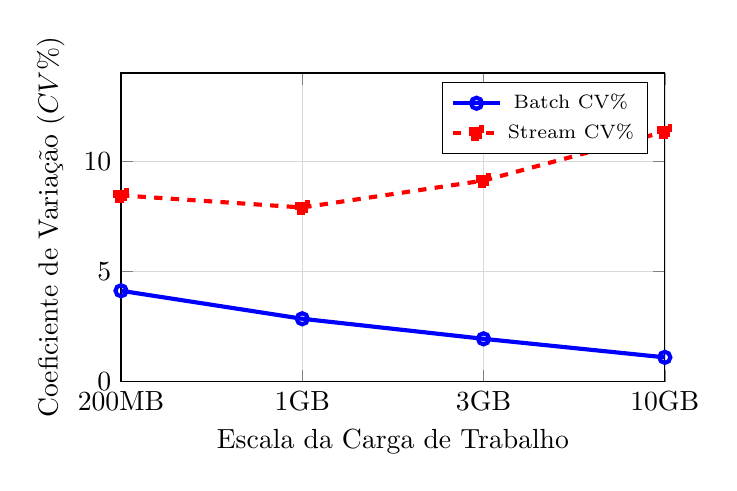
\begin{tikzpicture}
\begin{axis}[
    width=0.7\textwidth,
    height=5.5cm,
    xmin=0, xmax=3,
    xtick={0,1,2,3},
    xticklabels={200MB, 1GB, 3GB, 10GB},
    xlabel={Escala da Carga de Trabalho},
    ymin=0, ymax=14,
    ylabel={Coeficiente de Variação ($CV\%$)},
    grid=both,
    grid style={line width=.1pt, draw=gray!10},
    major grid style={line width=.2pt, draw=gray!30},
    legend pos=north east,
    legend style={font=\scriptsize}
]
% Linha do Batch
\addplot[color=blue, mark=o, thick, line width=1.5pt] coordinates {
    (0, 4.12) (1, 2.85) (2, 1.94) (3, 1.10)
}; \addlegendentry{Batch CV\%}

% Linha do Stream
\addplot[color=red, mark=square*, dashed, thick, line width=1.5pt] coordinates {
    (0, 8.45) (1, 7.90) (2, 9.12) (3, 11.34)
}; \addlegendentry{Stream CV\%}
\end{axis}
\end{tikzpicture}
\caption{Evolução da variabilidade operacional ($CV\%$) conforme a escala de carga (RQ2).}
\label{fig:rq2_variabilidade}
\end{figure}

A análise conjunta dos dados e do comportamento gráfico revela um fenômeno de divergência estrutural entre as duas abordagens arquiteturais. No paradigma \textit{batch}, constata-se que o aumento volumétrico atua como um fator de estabilização do cluster. À medida que a carga de dados cresce de 200MB para 10GB, o valor do $CV\%$ decresce de forma contínua, caindo de $4{,}12\%$ para meros $1{,}10\%$. 

Este comportamento é explicado pela amortização eficiente dos custos fixos computacionais em sistemas distribuídos. Cargas muito pequenas sofrem uma penalização proporcional elevada decorrente do \textit{overhead} de inicialização do ecossistema Spark, alocação de JVMs, registro de \textit{executors} e coordenação inicial do \textit{Task Scheduler}. Quando o volume de dados se torna massivo, o tempo gasto com o processamento real da carga domina a execução sobre os custos fixos de gerência, resultando em uma operação altamente previsível, estável e com baixa dispersão estatística.

Em contrapartida, o paradigma \textit{streaming} exibe uma curva de instabilidade ascendente. Embora ocorra uma leve oscilação positiva na transição inicial para 1GB ($7{,}90\%$), o avanço para volumes de 3GB e 10GB eleva o Coeficiente de Variação para $9{,}12\%$ e $11{,}34\%$, respectivamente. 

Este ganho de volatilidade indica que o escalonamento volumétrico em pipelines contínuos penaliza a consistência temporal da computação. Sob cargas elevadas, os nós do cluster enfrentam gargalos cumulativos na camada de rede (ingestão via tópicos do Apache Kafka), saturação de memória física durante as operações de agrupamento em micro-lotes e atrasos recorrentes na persistência dos metadados de \textit{checkpointing}. Essa disputa intensa por recursos computacionais gera picos localizados de latência e variações de processamento entre as janelas temporais, o que degrada a estabilidade macroscópica do sistema e eleva a incerteza operacional da arquitetura de fluxo contínuo.

\subsection{RQ3 --- Intervalos de Trigger e Latência de Eventos}
Na terceira questão de pesquisa experimental (RQ3), restringiu-se o escopo de análise ao ecossistema de processamento contínuo (\textit{streaming}) com o objetivo de mensurar as consequências operacionais da parametrização temporal dos gatilhos de execução (\textit{triggers}). Para determinar o impacto dessas variações de configuração, aplicou-se o teste não-paramétrico de Kruskal-Wallis. O modelo estatístico validou de forma robusta que a alteração programática do intervalo de \textit{trigger} resulta em modificações estatisticamente significativas nas métricas de latência e estabilidade do \textit{Spark Structured Streaming} ($p < 0{,}001$). 

A Tabela~\ref{tab:rq3_operational} consolida as variáveis de desempenho capturadas durante as sessões controladas sob os intervalos amostrais de $1\text{s}$, $2\text{s}$ e $5\text{s}$.

\begin{table}[htbp]
\centering
\caption{Métricas operacionais de streaming segmentadas por intervalo de trigger (RQ3).}
\label{tab:rq3_operational}
\small
\setlength{\tabcolsep}{5pt}
\begin{tabular}{lccccc}
\toprule
\textbf{Cenário} & \textbf{\shortstack{Lat. Trigger\\(ms)}} & \textbf{\shortstack{Lat. Evento\\(s)}} & \textbf{\shortstack{Backpressure\\(ms)}} & \textbf{\shortstack{Throughput\\(linhas/s)}} & \textbf{\shortstack{Jitter\\(ms)}} \\
\midrule
ST1 (1s) & 1464,70 & 1,42 & 240,10 & 745,20 & 75,90 \\
ST2 (2s) & 1828,00 & 2,15 & 115,40 & 742,10 & 122,90 \\
ST3 (5s) & 2571,00 & 5,60 & 42,80  & 739,80 & 152,60 \\
\bottomrule
\end{tabular}
\vspace{0.3em}
\begin{flushleft}
\footnotesize Fonte: elaborado pelo autor.
\end{flushleft}
\end{table}

A Figura~\ref{fig:rq3_tradeoff} ilustra graficamente o comportamento oposto da latência do evento em relação ao tempo de barramento reprimido (\textit{backpressure}), servindo como subsídio visual para o mapeamento de gargalos.

\begin{figure}[htbp]
\centering
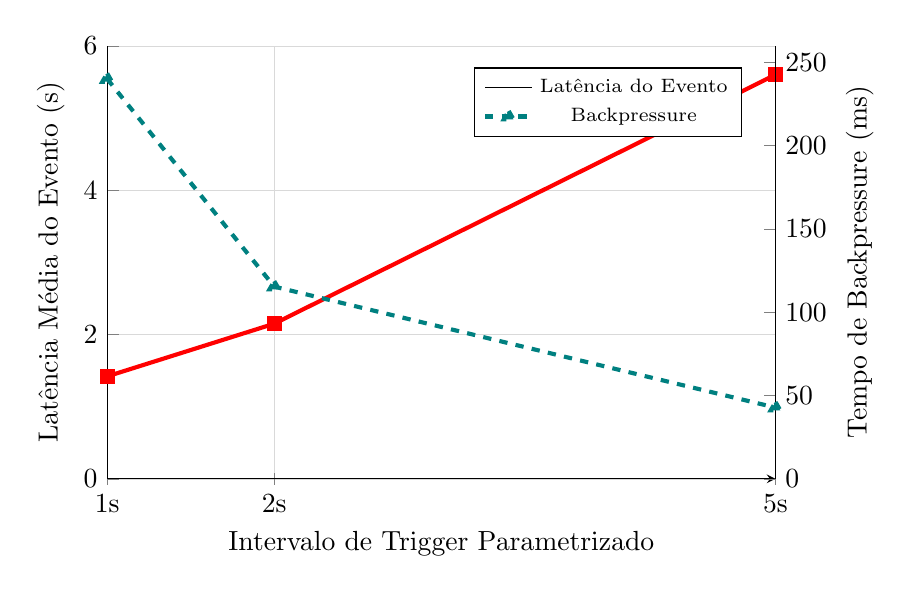
\begin{tikzpicture}
% CONFIGURAÇÃO DO PRIMEIRO EIXO (Esquerda - Latência do Evento)
\begin{axis}[
    scale only axis,
    width=0.7\textwidth,
    height=5.5cm,
    xmin=1, xmax=5,
    xtick={1,2,5},
    xticklabels={1s, 2s, 5s},
    xlabel={Intervalo de Trigger Parametrizado},
    ymin=0, ymax=6,
    ylabel={Latência Média do Evento (s)},
    axis y line*=left,
    axis x line=bottom,
    grid=both,
    grid style={line width=.1pt, draw=gray!10},
    major grid style={line width=.2pt, draw=gray!30}
]
\addplot[color=red, mark=square*, thick, line width=1.5pt] coordinates {
    (1, 1.42) (2, 2.15) (5, 5.60)
}; \label{plot:latencia}
\end{axis}

% CONFIGURAÇÃO DO SEGUNDO EIXO (Direita - Backpressure)
\begin{axis}[
    scale only axis,
    width=0.7\textwidth,
    height=5.5cm,
    xmin=1, xmax=5,
    ymin=0, ymax=260,
    ylabel={Tempo de Backpressure (ms)},
    axis y line*=right,
    axis x line=none,
    xtick=\empty,
    axis background/.style={fill=none}, 
    legend style={at={(0.95,0.95)}, anchor=north east, font=\scriptsize}
]

\addlegendimage{/pgfplots/refstyle=plot:latencia}\addlegendentry{Latência do Evento}

\addplot[color=teal, mark=triangle*, dashed, thick, line width=1.5pt] coordinates {
    (1, 240.10) (2, 115.40) (5, 42.80)
}; \addlegendentry{Backpressure}
\end{axis}
\end{tikzpicture}
\caption{Dilema arquitetural (trade-off) entre latência do evento e backpressure operacional (RQ3).}
\label{fig:rq3_tradeoff}
\end{figure}

Os dados empíricos e as curvas expostas revelam um \textit{trade-off} crítico de design arquitetural para engenharia de software de fluxos de dados. Observa-se que a dilatação deliberada do intervalo de gatilho de $1\text{s}$ para $5\text{s}$ atua de forma eficaz na mitigação da pressão imediata exercida sobre as filas de ingestão do sistema. Esse fenômeno é evidenciado pela redução drástica no tempo médio de interrupção por \textit{backpressure}, que cai de $240{,}10\text{ms}$ para meros $42{,}80\text{ms}$. Ao espaçar as execuções, o motor de micro-lotes ganha janelas mais folgadas para processar as mensagens retidas no Apache Kafka, reduzindo a concorrência imediata de escrita e o estresse sobre os buffers internos de memória do cluster.

Contudo, este alívio operacional impõe uma penalidade severa sobre os requisitos não-funcionais de reatividade e previsibilidade temporal do sistema. A latência média acumulada do evento sofre uma degradação expressiva, saltando de $1{,}42\text{s}$ para $5{,}60\text{s}$. Esse atraso é acompanhado por uma ampliação acentuada na instabilidade temporal da entrega dos dados (\textit{jitter}), que duplica de $75{,}90\text{ms}$ para $152{,}60\text{ms}$, sinalizando um comportamento de processamento altamente irregular e em rajadas (\textit{bursty}).

Adicionalmente, constata-se que a estratégia de acumular um volume maior de registros por ciclo (\textit{micro-batching} expandido) não se reverteu em ganhos de eficiência de vazão computacional, uma vez que o \textit{throughput} bruto permaneceu praticamente estagnado na faixa de 740 linhas por segundo em todos os cenários. Do ponto de vista de design de arquitetura de software, essa descoberta demonstra que a parametrização do \textit{trigger} não funciona como uma alavanca para o aumento de capacidade de vazão máxima, configurando-se estritamente como um botão de sintonia fina para equilibrar a tolerância a picos de carga contra a necessidade de processamento em tempo real estrito.

\subsection{RQ4 --- Escalabilidade Horizontal e Eficiência Arquitetural}
Na quarta questão de pesquisa (RQ4), avaliou-se a capacidade de resposta de ambos os paradigmas diante da expansão da infraestrutura computacional utilizando clusters com 1, 2 e 4 instâncias operacionais (\textit{workers}) sob a carga máxima de 10GB. Para quantificar a eficiência de paralelização, foram computadas as métricas de Speedup Observado ($S$) e Eficiência de Escalonamento ($E$), cujos resultados estão expostos na Tabela~\ref{tab:rq4_scalability_metrics}.

\begin{table}[htbp]
\centering
\caption{Métricas de escalabilidade e eficiência de paralelização no cluster (RQ4).}
\label{tab:rq4_scalability_metrics}
\small
\setlength{\tabcolsep}{6pt}
\begin{tabular}{lccccc}
\toprule
\textbf{Paradigma} & \textbf{Workers} & \textbf{Throughput Médio} & \textbf{Comportamento} & \textbf{Speedup ($S$)} & \textbf{Eficiência ($E$)} \\
\midrule
\textbf{Batch}   & 1 & 20,67 M linhas/s & Linha de Base  & 1,00 & 1,00 \\
                 & 2 & 29,67 M linhas/s & Sublinear      & 1,44 & 0,72 \\
                 & 4 & 30,92 M linhas/s & Saturação      & 1,50 & 0,38 \\
\midrule
\textbf{Stream}  & 1 & 1264,00 linhas/s & Linha de Base  & 1,00 & 1,00 \\
                 & 2 & 1220,00 linhas/s & Degradação     & 0,96 & 0,48 \\
                 & 4 & 1172,00 linhas/s & Ineficiência   & 0,93 & 0,23 \\
\bottomrule
\end{tabular}
\vspace{0.3em}
\begin{flushleft}
\footnotesize Fonte: elaborado pelo autor.
\end{flushleft}
\end{table}

A divergência estrutural entre as duas abordagens é evidente. O processamento \textit{batch} demonstra ganho positivo de escalabilidade horizontal ao expandir de 1 para 2 \textit{workers} ($S = 1{,}44$). Contudo, atinge um patamar de saturação precoce em 4 \textit{workers} ($S = 1{,}50$), onde a eficácia computacional cai para $38\%$, indicando que a sobrecarga distribuída de particionamento e coordenação passa a anular os benefícios do acréscimo de hardware.

No paradigma de \textit{streaming}, constata-se um cenário de escalabilidade negativa. A inserção de novos nós de processamento causou regressão no \textit{throughput} absoluto (reduzindo de 1264 para 1172 linhas/s em 4 \textit{workers}), derrubando a eficiência do cluster para pífios $23\%$. Esse comportamento deletério indica que a sobrecarga contínua associada à coordenação dos estágios, sincronização de \textit{offsets} no Apache Kafka e gestão de estado distribuído sob o modelo de micro-lotes impõe barreiras severas ao paralelismo horizontal. Esse fenômeno é mapeado comparativamente contra a linha ideal linear na Figura~\ref{fig:rq4_speedup_chart}.

\begin{figure}[htbp]
\centering
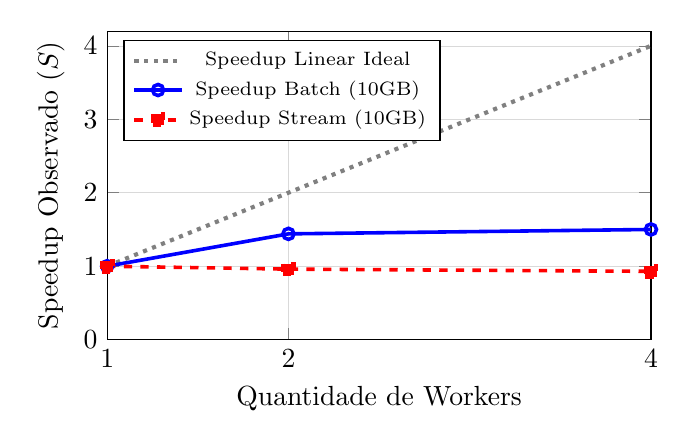
\begin{tikzpicture}
\begin{axis} [
    width=0.7\textwidth,
    height=5.5cm,
    xlabel={Quantidade de Workers},
    ylabel={Speedup Observado ($S$)},
    xmin=1, xmax=4,
    ymin=0, ymax=4.2,
    xtick={1,2,4},
    grid=both,
    grid style={line width=.1pt, draw=gray!10},
    major grid style={line width=.2pt, draw=gray!30},
    legend pos=north west,
    legend style={font=\scriptsize}
]
\addplot[color=gray, dotted, line width=1.5pt] coordinates {
    (1, 1) (2, 2) (4, 4)
}; \addlegendentry{Speedup Linear Ideal}

\addplot[color=blue, mark=o, thick, line width=1.3pt] coordinates {
    (1, 1.00) (2, 1.44) (4, 1.50)
}; \addlegendentry{Speedup Batch (10GB)}

\addplot[color=red, mark=square*, dashed, thick, line width=1.3pt] coordinates {
    (1, 1.00) (2, 0.96) (4, 0.93)
}; \addlegendentry{Speedup Stream (10GB)}
\end{axis}
\end{tikzpicture}
\caption{Curvas de speedup experimental frente ao limite linear ideal (RQ4).}
\label{fig:rq4_speedup_chart}
\end{figure}

A Tabela~\ref{tab:sintese-resultados-parciais} sintetiza as descobertas obtidas até o momento nas frentes de investigação mapeadas, servindo como base estrutural para a consolidação do modelo conceitual.

\begin{table}[htbp]
\centering
\caption{Síntese dos resultados parciais e implicações arquiteturais.}
\label{tab:sintese-resultados-parciais}
\scriptsize
\setlength{\tabcolsep}{4pt}
\renewcommand{\arraystretch}{1.3}
\begin{tabularx}{\textwidth}{lXX}
\toprule
\textbf{Dimensão Analisada} & \textbf{Resultado Parcial Consolidado} & \textbf{Implicação para o Modelo de Decisão} \\
\midrule
Revisão Sistemática & 10 estudos primários preencheram integralmente os critérios de elegibilidade e qualidade. & O volume reduzido evidencia a fragmentação de dados concretos para o design de sistemas intensivos em dados. \\
\midrule
Síntese Quantitativa & As otimizações arquiteturais exibiram efeito médio positivo ($\overline{\text{LRR}} = 0{,}981$), com razão de resposta de $\approx 2{,}7\times$. & Há indícios robustos de ganhos empíricos, mas as evidências na literatura carecem de padronização nos relatos estatísticos. \\
\midrule
RQ1 --- Batch vs Streaming & O paradigma \textit{batch} demonstrou superioridade de vazão em ordens de magnitude na comparação direta. & A escolha do paradigma deve priorizar os requisitos não-funcionais: maximização de throughput bruto (\textit{batch}) vs menor latência temporal (\textit{stream}). \\
\midrule
RQ2 --- Volume de Dados & O volume determinou a estabilização estatística do \textit{batch} ($CV = 1{,}10\%$) e o aumento de instabilidade do \textit{stream} ($CV = 11{,}34\%$). & O volume de dados bruto deve atuar como variável de entrada ponderada na matriz de decisão da arquitetura. \\
\midrule
RQ3 --- Triggers & O escalonamento do trigger (1s para 5s) mitigou o backpressure ($240\text{ms}$ para $42\text{ms}$), mas dobrou o jitter ($75\text{ms}$ para $152\text{ms}$). & Configurações de micro-lotes introduzem trade-offs matemáticos inevitáveis entre estabilidade temporal e vazão. \\
\midrule
RQ4 --- Escalabilidade & A adição de workers saturou o \textit{batch} ($E = 0{,}38$) e causou regressão de desempenho no \textit{streaming} ($E = 0{,}23$). & A infraestrutura horizontal não garante ganhos automáticos e depende da sensibilidade do paradigma ao overhead distribuído. \\
\bottomrule
\end{tabularx}
\vspace{0.3em}
\begin{flushleft}
\footnotesize Fonte: elaborado pelo autor.
\end{flushleft}
\end{table}

O mapeamento empírico consolidado na Tabela~\ref{tab:sintese-resultados-parciais} evidencia que a engenharia de sistemas intensivos em dados não pode se apoiar em premissas simplistas de escalonamento linear. Os comportamentos observados nas quatro questões de pesquisa demonstram que variáveis de infraestrutura (como a adição de \textit{workers}) e de configuração de \textit{runtime} (como intervalos de \textit{trigger}) desencadeiam reações severas e frequentemente contra-intuitivas na estabilidade e na vazão das arquiteturas distribuídas. A constatação de uma eficiência de paralelização decrescente no modelo \textit{batch} ($E = 0{,}38$) e abertamente regressiva no modelo de \textit{streaming} ($E = 0{,}23$) corrobora a necessidade de uma abordagem analítica formal para guiar decisões de design de software antes da alocação massiva de recursos computacionais.

Essa interdependência de fatores técnicos justifica a relevância de se unificar os achados empíricos em um arcabouço metodológico estruturado. Os dados de variabilidade da RQ2 e os \textit{trade-offs} temporais da RQ3 isolam os limiares operacionais onde cada paradigma deixa de ser eficiente. Consequentemente, essas métricas deixam de ser meros indicadores de desempenho passivos e passam a atuar como os parâmetros de entrada quantitativos indispensáveis para a calibração do modelo de decisão arquitetural proposto nesta pesquisa.


\section{Integração dos Resultados}
\label{sec:integracao-resultados}

Os resultados parciais da revisão sistemática e da campanha experimental convergem para uma mesma conclusão: decisões arquiteturais em sistemas intensivos em dados dependem fortemente do contexto. A literatura mostra que diferentes técnicas podem produzir ganhos relevantes, mas tais ganhos estão intrinsecamente associados a características específicas de \textit{workloads}, ambientes e métricas escolhidas. A campanha experimental, por sua vez, comprova que a escolha entre \textit{batch} e \textit{streaming}, bem como a configuração de paralelismo e \textit{trigger}, produz efeitos distintos sobre \textit{throughput}, latência, escalabilidade e estabilidade.

Essa convergência sustenta a necessidade de uma abordagem de apoio à decisão arquitetural. Em vez de assumir que uma técnica ou paradigma é universalmente superior, a decisão deve ponderar as características dos dados, os requisitos de desempenho e as restrições operacionais do sistema.

A principal contribuição dos resultados parciais reside na identificação de relações entre fatores arquiteturais e métricas observáveis. A Revisão Sistemática da Literatura indica que ganhos de desempenho podem ser obtidos em diferentes camadas do sistema. A campanha experimental demonstra que decisões como escolha do paradigma, variação do volume, ajuste de \textit{trigger} e aumento do número de \textit{workers} geram efeitos discrepantes dependendo do contexto operacional.



\section{Implicações para o Modelo de Apoio à Decisão}
\label{sec:implicacoes-modelo}

Os resultados obtidos até o momento fornecem insumos fundamentais para a especificação do modelo proposto. A Revisão Sistemática da Literatura indica quais tipos de decisões arquiteturais têm sido formalmente investigadas e quais métricas são adotadas para avaliá-las. A campanha experimental fornece evidências controladas sobre como fatores como volume, taxa de eventos, paralelismo e intervalo de \textit{trigger} degradam ou otimizam o comportamento de um \textit{pipeline} baseado em Apache Spark e Apache Kafka.

Esses resultados sugerem que o modelo de apoio à decisão deve incorporar múltiplas dimensões, destacando-se:
\begin{itemize}
    \item \textbf{Características dos dados:} tais como volume, distribuição, redundância e entropia;
    \item \textbf{Características da carga:} como taxa de eventos e variabilidade temporal;
    \item \textbf{Requisitos arquiteturais:} incluindo latência máxima aceitável e \textit{throughput} mínimo esperado;
    \item \textbf{Configurações operacionais:} como número de \textit{workers} e intervalo de \textit{trigger};
    \item \textbf{Métricas de custo computacional:} tais como perfil de uso de CPU, memória, rede e operações de disco.
\end{itemize}

Dessa forma, os resultados parciais não apenas respondem às questões iniciais da revisão e da campanha experimental, mas auxiliam na delimitação dos elementos que deverão compor a próxima etapa metodológica da pesquisa. Esses achados reforçam a necessidade de uma abordagem de apoio à decisão arquitetural que considere evidências empíricas, características intrínsecas dos dados e requisitos de desempenho, avançando além de recomendações genéricas ou dependentes exclusivamente da intuição do arquiteto de software.
